\section{Dependency Parsing (DP) using MTT}

\subsection*{Goal} Construct dependency tree (DT) with syntactic relations, e.g., noun-modifier, determiner, etc. DT is a directed spanning(every node on graph connected) tree, with an additional root node having $\mathrm{deg}_{\mathrm{out}}=1$.

\subsection*{Relation to context free grammar}
CFG: no information on syntactic relation; DP: no information on constituency structure. 

\subsection*{Methods for cauculating Partition Function} 
(1) Projective DT: no crossing arcs. Equivalent to lexicalized CFG. Algorithms are generally dynamic programming. \\
(2) Non-Projective DT: crossing arcs. Algorithms use matrix-tree theorem (MTT).


\subsection*{$\mathcal{Z}$ for Non-Proj DT in Edge-Factored Assump}
Assume $p(\mathbf{t} \mid \mathbf{w})=\frac{1}{Z} \prod_{(i \rightarrow j) \in \mathbf{t}} \exp \{\operatorname{score}(i\to j, \mathbf{w})\} \exp \{\operatorname{score}(\mathrm{root}, \mathbf{w})\}$.

Def: edge score $A_{ij}=\exp(\score(i,j,w))$, root score $\rho_j = \exp(\score(j,w))$. \textbf{MTT} says $Z=|L|$ for following $L$ which is $O(n^3)$:
\vspace{-0.3cm}
$$L_{i j}= \begin{cases}-A_{i j} & \text { if } i \neq j \\ \rho_{j}+\sum_{k \neq i} A_{k j} & \text { otherwise }\end{cases}$$
\vspace{-0.3cm}

\subsection*{Decoding the best DT}
Find the best directed spanning tree starting from root and the degree of root is 1. \; Kruskal's algorithms (greedy) that work in undirected graph do not work.

Chu-Liu-Edmonds Algo ($O(n^3)$, optimized to $O(n^2)$ by Tarjan): \quad
(1) Find the best \emph{incoming} edge for each vertex. 
(2) Contract cycles to be a single node $c$ and increase the weight of incomming edge by $c.n_{i}$ with $w(c.n_{i}\to c.n_{i+1})+\cdots$ until the last node in the circle. 
(3) Continue contraction until $\mathcal{G}$ has a spanning tree. 

\vspace{-0.4cm}
\begin{center}
    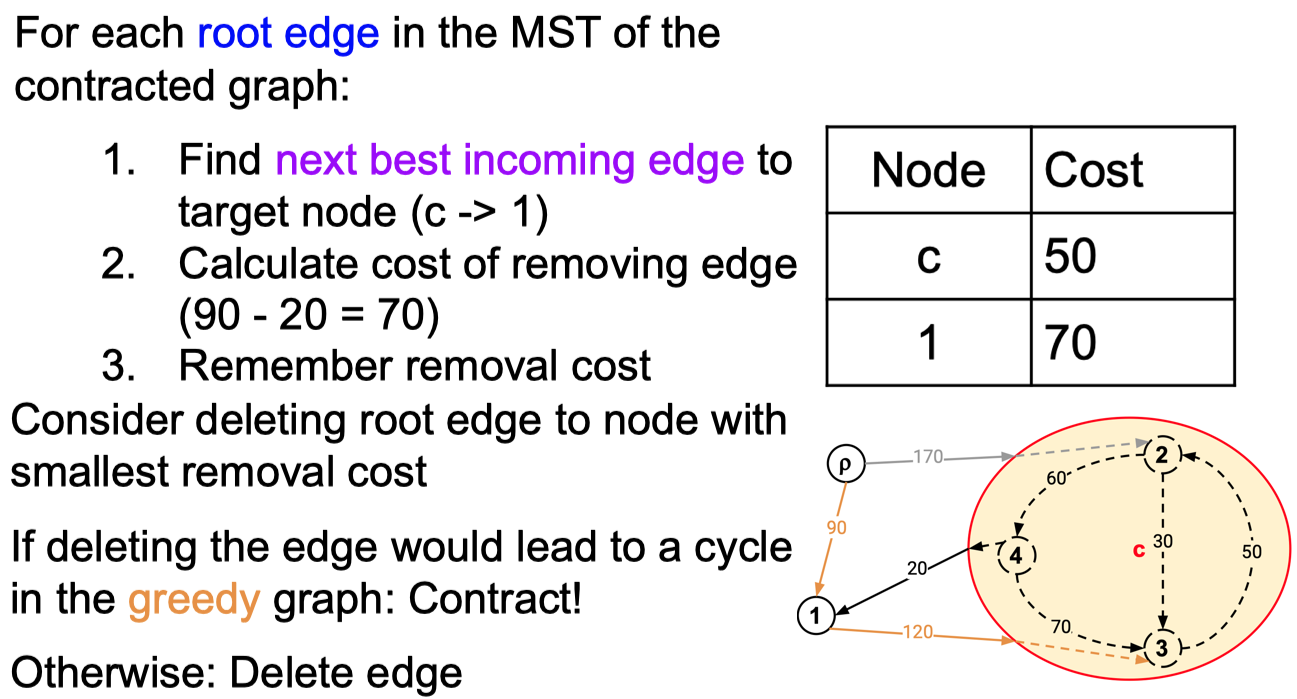
\includegraphics[width=\columnwidth]{img/root-remove.png}
\end{center}
\vspace{-0.5cm}

(4) Expand contract nodes by breaking cycles accordingly.
